\section{Description of the Model}
\subsection{Basic model: Hive simulation}
	Our model is widely based on the studies and equations of Khoury et al. \cite{khoury13}. Food, seasons, brood, foragers and hive bees are the cornerstone of our model. The dynamics of the hive is based on the bee's behaviour and their interaction with the environment as well as natural influences, i.e. seasons (see Fig X). Food here means nectar and pollen, which is not further distinguished for simplicity reasons. There are only female bees since they are responsible for the foraging process and the maintenance and sustainability of the population. After the queen laid an egg, a larvae develops inside a honeycomb cell. The equations show the proportionality of the pupation to the food income. Neglecting the complicated process of becoming an adult bee, we assume that larvae become hive bees 12 days after pupation. The mortality rate of hive bees and capped brood is negligible if we do not implement specific infecting diseases. With all these information we can set up
	
	\begin{equation}\label{rate of change of brood numbers}
		{dB \over dt} = LS(H,f)-\phi B
	\end{equation}
	
	representing the rate of change of brood numbers, where $L$ is the laying rate of the bee queen, $S(H,f)$ is the survival rate, a function dependent on the number of hive bees and the amount of food available. $\phi$ is the adult bee emerging factor and $B$ represents the uncapped brood. The equation gives us the survival rate pf the brood. $S(H,f)$ is modelled as following:
	
	\begin{equation}\label{function of hive bees and food}
		S(H,f)={f^2 \over f^2+b^2}{H \over H+v}
	\end{equation}
	
	$v$ indicated the effect of the hive bees on the brood, whereas $b$ shows the food effect on brood survival. It decreases as food increases. As $f$ and $H$ become very large, $S(H,f)$ becomes constant. The food and hive bee number is no longer connected to each other. The first factor is a sigmoid function and shows the correlation of the food available and the capped brood. A decrease in brood can occur because of a lack of food, they cannot be fed, and because adult bees consume the larvae to keep the resources in the hive and recycle the proteins. The second factor models the interdependency of the hive bee numbers on the survival of the brood. If there are large stores of food but no hive bees that can provide the food to the larvae, the brood survival declines.  
	\\
	The second differential equation describes the rate of change of hive bees:
	
	\begin{equation}
		{dH \over dt}=\phi B(t-\tau)-HR(H,F,f)
	\end{equation}
	
	$\tau$ is the ageing time and the whole product $\phi B(t-\tau)$ is the rate at which adult bees hatch out from pupation. The second term is explained below.\\ 
	The third differential equation describes the rate of change of foragers
	
	\begin{equation}\label{Rate of change of foragers}
		{dF \over dt} = HR(H,F,f)-m F
	\end{equation}
	
	with the recruitment function
	
	\begin{equation}\label{rate of change of foragers }
		HR(H,F,f) = \alpha_{min} + \alpha_{max}({b^2 \over b^2+f^2})-\sigma({F \over F+H})
	\end{equation}
	
	and the mortality rate $mF$. The recruitment function models the change from a hive bee to a forager bee. $\alpha_{min}$ denotes the transition when there is enough food but not much foragers. The rate is increased with less food described with $\alpha_{max}$. As before, $b$ is the food effect on brood survival and $f$ is the amount of food. $\sigma$ is the strength of social inhibition and is dependent on the number of foragers and hive bees.\\
	Rate of change in food stores:
	
	\begin{equation}\label{Rate of change in food stores}
		{df \over dt} = c F - \gamma_A (F+H) - \gamma_B B
	\end{equation}
	
	% This is actually wrong, we did not change c in our (basic) model... have a look at the code. In the advanced model, we replace the term c * F with the result from the actual environment simulation! Please correct.
	where $c$ describes the average food a single forager collects per day. In contrast to Khoury, we implemented also a seasonal dependent factor, so c changes with rate X over time. $\gamma$ is the consumption of adult bees ($A$) and brood ($B$). It is not differentiated between foragers and hive bees.  

	\subsection{Changing laying rate over seasons}
		\begin{figure}
			\centering
			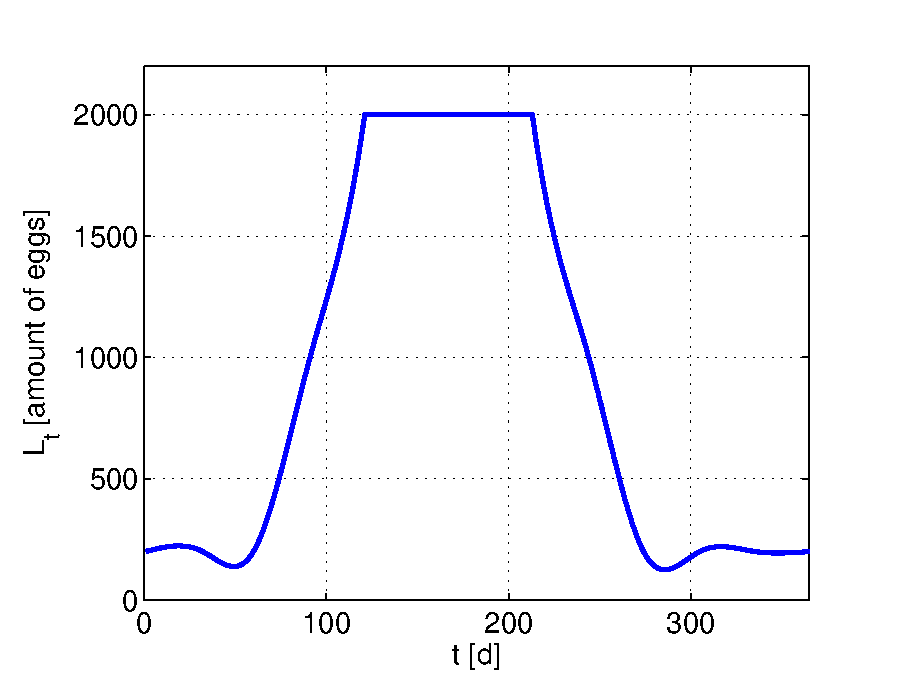
\includegraphics{data/egg_plot.eps}
			\caption{The laying rate of the bee queen plotted over a year. The amount of eggs is capped after 2000 eggs.}
			% http://www.beesource.com/point-of-view/walt-wright/how-many-eggs-can-a-queen-lay
			% TODO: Rearrange/put link somewhere else
		\end{figure}
		
		% TODO: Description of what changed here!
		
		\begin{equation}\label{rate of change of brood numbers over time}
			{dB \over dt} = L(t)S(H,f)-\phi B
		\end{equation}
	
	\subsection{Advanced model: Environment simulation}
		\subsubsection{Bees' working states}
		\subsubsection{Foragers' distribution across flower patches}
	\subsection{Empirical data bases}


